\documentclass{clv2025}

\jvol{vv}
\jnum{nn}
\jyear{2026}
\jinfo{}
\renewcommand{\footmark}{}
\dochead{Position Paper}

\usepackage[T1]{fontenc}
\usepackage[american]{babel}
\usepackage{natbib}
\bibliographystyle{compling}
\usepackage{mathtools}
\usepackage{amssymb}
\usepackage{booktabs}
\usepackage{tabularx}
\usepackage{array}
\usepackage{graphicx}
\usepackage{xcolor}
\usepackage{tikz}
\usetikzlibrary{arrows.meta,positioning,calc}
\hypersetup{hidelinks}

\newcommand{\TC}{\textsc{TC}}
\newcommand{\LD}{\textsc{LD}}
\newcommand{\Hall}{\textsc{H}}
\newcommand{\SUP}{\textsc{SUP}}
\newcommand{\SV}{\textsc{SV}}
\newcolumntype{Y}{>{\raggedright\arraybackslash}X}
\newcolumntype{P}[1]{>{\raggedright\arraybackslash}p{#1}}

\definecolor{clrH}{RGB}{155,18,18}
\definecolor{clrLD}{RGB}{22,98,48}
\definecolor{clrB}{RGB}{22,52,125}
\definecolor{clrG}{RGB}{65,65,65}
\definecolor{bgB}{RGB}{245,247,254}
\tikzset{
  input/.style={rectangle,rounded corners=4pt,draw=gray!55,fill=gray!8,
    font=\small\itshape,text width=5.0cm,align=center,inner sep=6pt},
  decision/.style={rectangle,rounded corners=3pt,draw=clrB!55,fill=bgB,
    font=\small,text width=5.2cm,align=center,inner sep=6pt},
  verdict/.style={rectangle,rounded corners=3pt,draw=clrG,fill=gray!8,
    font=\small\bfseries\sffamily,inner xsep=7pt,inner ysep=4pt},
  verdictH/.style={verdict,draw=clrH,text=clrH,fill=clrH!7},
  verdictLD/.style={verdict,draw=clrLD,text=clrLD,fill=clrLD!7},
  arrow/.style={-{Stealth[length=5pt,width=3.5pt]},thick,color=gray!70!black},
  edge/.style={font=\scriptsize\sffamily,fill=white,inner sep=1.5pt}
}

\title{Hallucination Is Task-Relative: A Truth-Contract Framework for Evaluating LLM Outputs}
\runningtitle{Hallucination Is Task-Relative}
\runningauthor{Carlesso et al.}

\author{Mathis Carlesso$^{1,2}$, Martino Lovisetto$^{2}$, El\H{o}d Egyed-Zsigmond$^{1}$, Pierre-Yves Genest$^{2}$, Stefan Duffner$^{1}$}

\affilblock{
  \affil{INSA Lyon, CNRS, LIRIS, UMR5205, Universit\'e Claude Bernard Lyon 1, 69621 Villeurbanne, France\\
  \quad \email{mathis.carlesso@insa-lyon.fr}}
  \affil{Alteca, 69100 Villeurbanne, France}
}

\begin{document}
\maketitle

\begin{abstract}
Hallucination in large language models is usually defined as unsupported or contradicted content.
This definition fits factual reporting, but it becomes ambiguous when a task allows invention or asks for figurative language.
We argue that hallucination should instead be a claim-level verdict relative to a task's \emph{truth contract}, $\TC(p)=(O_p,\sigma_p,K_p)$.
The contract specifies the reference evidence $O_p$, the requested style level $\sigma_p$, and the content-permission policy $K_p$.
Within $K_p$, a permission level $\kappa_p\in\{0,1,2\}$ distinguishes factual-only tasks, limited and explicitly marked divergence, and invention inside a declared frame; the policy also specifies where and how such divergence is allowed.
The evaluator first separates factual claims from stylistic wording and then checks only the extracted claims.
A supported claim receives \SUP; a contradicted or unlicensed claim receives \Hall; and an evidence-unknown claim receives \LD\ only when the task permits it within scope and it is presented as required.
The style level guides the interpretation of metaphors and other marked forms, but never permits unsupported content by itself.
This separation makes it possible to evaluate outputs that are creative in form while remaining factual when required.
We support the position with five worked cases and an author-coded mapping of forty evaluation resources.
In this sample, factuality benchmarks cluster around neutral language ($\sigma=0$) and factual-only permission ($\kappa=0$), whereas creative-writing benchmarks cluster around marked language ($\sigma=1$ or $2$) and task-implied invention ($\kappa=2$).
The two literatures therefore evaluate different truth contracts rather than conflicting versions of the same task.
The missing test is a controlled benchmark that varies style and permission independently.
\end{abstract}

\section{Introduction}\label{sec:intro}

Large language models (LLMs) can produce fluent claims that are unsupported by evidence or contradicted by known facts \citep{ji_survey_2023,huang_survey_2025}.
These errors limit the use of LLMs in high-stakes settings, and a large body of work aims to detect and reduce them \citep{lin_truthfulqa_2022,li_halueval_2023,wei_measuring_2024}.

However, unsupported generation is not always an error.
Fiction, brainstorming, and hypothesis generation require the model to go beyond established facts or provided documents \citep{franceschelli_creativity_2024,jiang_survey_2024,sui_confabulation_2024}.
A medical assistant should not invent a diagnosis.
A fiction-writing assistant must be able to invent characters and events.
The relevant distinction is therefore not only whether a statement is supported, but also whether the task permits that departure from support.

Many current evaluation protocols do not represent this distinction explicitly.
Factuality and faithfulness evaluations typically penalize unsupported claims under a fixed evidence source \citep{maynez_faithfulness_2020,bang_hallulens_2025}.
Creativity evaluations reward novelty and appropriateness, but they do not always test whether an apparently novel statement violates a factual constraint \citep{acar_creativity_2019,hou_creativityprism_2025}.
Consequently, two protocols can assign opposite verdicts to the same wording because each silently assumes a different task.

A second diagnostic problem concerns form rather than invention.
Stylistic foregrounding makes linguistic form salient through devices such as deviation, parallelism, metaphor, and unusual phrasing \citep{leech_short_style_1981,vanpeer_stylistics_2020}.
Some of these devices can change how a claim is expressed without adding a new factual commitment \citep{badathala_match_2023,jin_deep_2022}.
An evaluator that literalizes a metaphor, or reads surface unexpectedness as evidence of factual deviation, can therefore report a hallucination although the underlying claim remains supported.
The point is not that all current factuality systems make this error, but that many protocols do not expose requested style level as a variable with which the error can be measured.

\paragraph{Our position}
Hallucination is not a context-free property of a sentence.
It is a claim-level verdict relative to the task's truth contract, $\TC(p)=(O_p,\sigma_p,K_p)$.
The reference evidence $O_p$ specifies the standard of support.
The requested style level $\sigma_p$ specifies how strongly the prompt asks for departure from neutral wording, with factual commitments preserved.
The content-permission policy $K_p$ specifies the type, scope, and required epistemic presentation of any permitted departure.
An unsupported claim is \Hall\ if it violates $K_p$; an evidentially unknown claim is \LD\ if $K_p$ permits it and its presentation satisfies the contract.
The contract does not change what is true.
It determines whether the model's departure from the relevant evidence violates the task.

Figure~\ref{fig:flip} illustrates this position.
The example compares one surface sentence across two discourse frames.
It does not assume that the historical and fictional interpretations express the same contextualized claim.

\begin{figure}[t]
\centering
\resizebox{0.94\linewidth}{!}{%
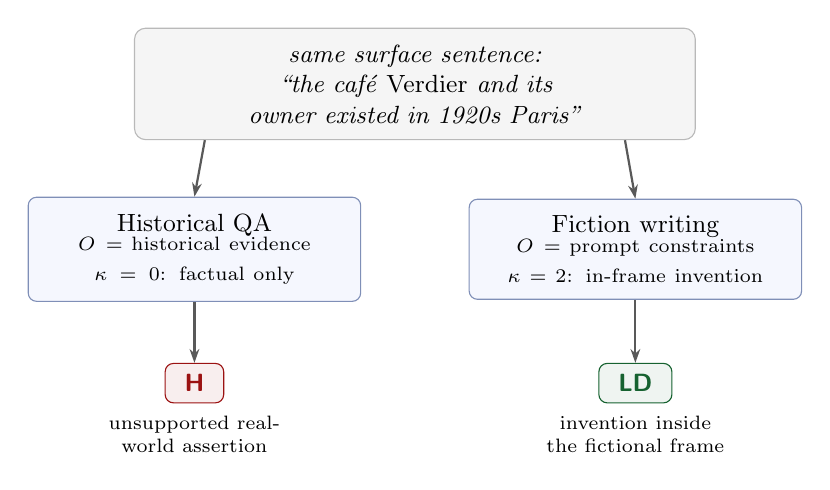
\begin{tikzpicture}[x=1cm,y=1cm]
  \node[input,text width=6.7cm] (s) at (0,0)
    {same surface sentence:\\``the caf\'e \emph{Verdier} and its owner existed in 1920s Paris''};
  \node[decision,text width=3.8cm] (qa) at (-2.8,-2.1)
    {Historical QA\\[-1pt]{\scriptsize $O=$ historical evidence\\$\kappa=0$: factual only}};
  \node[decision,text width=3.8cm] (fi) at (2.8,-2.1)
    {Fiction writing\\[-1pt]{\scriptsize $O=$ prompt constraints\\$\kappa=2$: in-frame invention}};
  \node[verdictH] (h) at (-2.8,-3.8) {\Hall};
  \node[verdictLD] (ld) at (2.8,-3.8) {\LD};
  \node[font=\scriptsize,align=center,text width=3.7cm] at (-2.8,-4.45)
    {unsupported real-world assertion};
  \node[font=\scriptsize,align=center,text width=3.7cm] at (2.8,-4.45)
    {invention inside the fictional frame};
  \draw[arrow] (s.south west) ++(0.9,0) -- (qa.north);
  \draw[arrow] (s.south east) ++(-0.9,0) -- (fi.north);
  \draw[arrow] (qa) -- (h);
  \draw[arrow] (fi) -- (ld);
\end{tikzpicture}}
\caption{\textbf{Contract-dependent evaluation of one surface sentence.}
In historical QA, the sentence is interpreted as a real-world claim and is unsupported under a grounded-only contract (\Hall).
In fiction writing, it is interpreted within the declared fictional world and falls inside the licensed scope (\LD).
Because the contextualized claims differ, the figure illustrates frame dependence rather than a same-claim label reversal.}
\label{fig:flip}
\end{figure}

\paragraph{Evidence and scope}
We support the position in two ways.
First, we map forty hallucination and creativity evaluation resources against the components of the proposed contract.
This purposive, author-coded mapping identifies a pattern in the sample rather than estimating prevalence in the full literature.
Second, we apply the decision rule to five worked cases involving reference evidence, the content-permission policy, epistemic presentation, scope, and $\sigma_p$-conditioned claim typing.
These cases illustrate the intended behavior of the rule but do not establish annotation reliability or completeness.

\paragraph{Contributions}
This position paper makes three contributions.
First, it introduces the truth contract $\TC(p)=(O_p,\sigma_p,K_p)$.
The contract separates reference evidence, requested style level, and the content-permission policy, and distinguishes \Hall\ from \LD.
Second, it maps a sample of factuality and creativity protocols to identify where task permissions and form-conditioned factuality checks remain implicit.
Third, it proposes a research agenda for contract-aware benchmarks and mitigation methods that reduce \Hall\ without suppressing \LD\ or factual stylistic creativity.

\section{Related Evaluation Paradigms}\label{sec:related}

Faithfulness asks whether a claim is supported by provided evidence, whereas factuality asks whether it is correct against an external reference \citep{maynez_faithfulness_2020,kryscinski_evaluating_2020}.
Both define evidence relations.
The content-permission policy asks a different question: what may an output do when the reference evidence does not entail a claim?

Intent-aware evaluation checks whether an output satisfies query constraints \citep{hao_faithqa_2025}.
This supports the broader view that hallucination evaluation should consider the task rather than the output alone.
However, general intent combines many requirements and does not isolate reference evidence, the content-permission policy, and epistemic presentation.

Recent work distinguishes potentially valuable or ``intelligent'' hallucinations from defective ones \citep{jiang_survey_2024,sui_confabulation_2024,yang_hicbench_2025}.
Our distinction does not rest on value.
Permission is evaluated first: an ingenious fabricated medical fact remains \Hall, whereas an unhelpful but in-frame fictional invention remains \LD\ with low usefulness.

Foregrounding and style-transfer research shows that marked form can be described and manipulated while attempting to preserve content \citep{leech_short_style_1981,vanpeer_stylistics_2020,pavlick_empirical_2016,rao_dear_2018,briakou_evaluating_2021}.
Hallucination evaluation, by contrast, focuses mainly on support and contradiction.
The missing bridge is a protocol that varies stylistic marking while holding the expressed claims and reference evidence fixed, then tests whether extraction and claim-level verdicts remain stable.

\section{Truth Contracts and Claim-Level Verdicts}\label{sec:framework}

\subsection{The truth contract}

\textbf{Truth contract (\TC).}
For prompt $p$, the truth contract is
\[
  \TC(p)=(O_p,\sigma_p,K_p), \qquad K_p=(\kappa_p,\Gamma_p,\rho_p).
\]
The three components answer different questions: what supports a claim, what style level the task requests, and what unsupported content the task permits.
We drop the subscript $p$ when the prompt is clear from context.

\textbf{Reference evidence ($O_p$).}
$O_p$ is the reference evidence against which a claim is evaluated, such as a source document, retrieval set, database, gold labels, or a specified external source.
The phrase ``world knowledge'' is only a shorthand; reproducible evaluation requires a concrete evidence source or an explicit adjudication procedure \citep{ji_survey_2023,bang_hallulens_2025}.

\textbf{Content-permission policy ($K_p$).}
$K_p$ specifies three properties:
\begin{itemize}
  \item $\kappa_p\in\{0,1,2\}$: the permission level, where $0$ is factual only, $1$ allows limited and explicitly marked divergence, and $2$ allows invention inside a declared frame;
  \item $\Gamma_p$: the scope within which unsupported content is allowed;
  \item $\rho_p$: the required epistemic presentation, such as a hedge, an explicit hypothesis marker, or a declared fictional frame.
\end{itemize}
The scale orders only the breadth of permitted departure from the reference evidence.
It is not a scale of quality, creativity, or factuality, and the number does not replace the scope and presentation constraints.
In particular, limited speculation and fiction carry different commitments and presentation requirements.

A grounded-only task has an empty permission scope for unsupported claims.
A hypothesis-generation task may allow claims within a stated topic if they are marked as provisional.
A fictional task may allow unhedged statements inside the declared fictional world while still prohibiting false claims about real people outside that frame \citep{searle_logical_1975}.

\subsection{Requested style levels}

The truth contract distinguishes three requested style levels, $\sigma_p\in\{0,1,2\}$:
\begin{itemize}
  \item $\sigma_p=0$ (neutral/literal): minimal rhetorical transformation and no salient authorial voice;
  \item $\sigma_p=1$ (moderately marked): local metaphor, register shift, or a light stylistic voice while the intended claims remain transparent;
  \item $\sigma_p=2$ (strongly marked): sustained figurative language, a salient voice, or substantial stylistic transformation.
\end{itemize}
The levels rank the degree of formal marking.
They do not rank creativity or factuality, and they do not grant permission to invent.
They operationalize \emph{foregrounding}: the prominence produced when a text departs from a neutral background through unexpected deviation or patterned regularity \citep{leech_short_style_1981,vanpeer_stylistics_2020}.
Metaphor is a central semantic case, but foregrounding may also be lexical, syntactic, phonological, or discourse-level.
Surface unexpectedness is therefore not, by itself, evidence of factual error.
Style is multi-dimensional, so this three-level scheme is a working discretization rather than a validated universal scale \citep{kang_style_2021,jin_deep_2022}.
The boundaries, especially between $\sigma_p=1$ and $\sigma_p=2$, require empirical validation.

The requested style level $\sigma_p$ must be distinguished from the observed style level $\widehat\sigma(s,p)$ in an output span $s$.
For example, a prompt can request $\sigma_p=2$ while the model produces neutral prose with $\widehat\sigma(s,p)=0$.
This mismatch is a style-compliance error, not a hallucination.

The diagnostic role of $\sigma_p$ is upstream of factual verification.
The requested style level guides the interpretation of a span, while the observed style level records the form that the model produced.
Claim extractors, entailment systems, and semantic metrics may react differently to literal and figurative realizations of the same claim \citep{chen_menli_2023,aynetdinov_semscore_2024,lai_multidimensional_2023,pauli_mind_2025}.
As a result, stylistic form can change which claims an evaluator extracts and verifies even though $\sigma_p$ does not authorize new content.

\subsection{Unit of analysis and span typing}

We use a claim-level unit because a response may mix supported, unsupported, and non-claim material \citep{min_factscore_2023,bayat_factbench_2024}.
Let $s$ denote a surface span and let $c(s,p)$ denote a truth-conditional claim obtained by interpreting $s$ in the context established by prompt $p$.
The same wording can yield different contextualized claims in fiction, metaphor, and hypothetical language.

Before assigning claim-level verdicts, the evaluator performs a contract-guided span analysis
\[
\mathcal X_{\sigma_p}(s,p)
=
\bigl(\mathcal C_{\sigma_p}(s,p),\widehat\sigma(s,p),z_{\sigma_p}(s,p)\bigr).
\]
Here, $\mathcal C_{\sigma_p}(s,p)$ is the set of extracted truth-conditional claims.
The observed style level $\widehat\sigma(s,p)\in\{0,1,2\}$ describes the produced form, and $z_{\sigma_p}(s,p)\in\{0,1\}$ marks an independently identifiable stylistic contribution (\SV).
This analysis produces four span types:
\begin{itemize}
  \item \emph{other}: $\mathcal C_{\sigma_p}=\varnothing$ and $z_{\sigma_p}=0$; the span is outside factual and stylistic evaluation;
  \item \emph{SV-only}: $\mathcal C_{\sigma_p}=\varnothing$ and $z_{\sigma_p}=1$; no factual claim is verified;
  \item \emph{claim-only}: $\mathcal C_{\sigma_p}\neq\varnothing$ and $z_{\sigma_p}=0$; each extracted claim is verified;
  \item \emph{mixed}: $\mathcal C_{\sigma_p}\neq\varnothing$ and $z_{\sigma_p}=1$; the span keeps \SV\ while each claim is verified.
\end{itemize}
Metaphor is not automatically removed from factual evaluation.
We annotate a metaphorical span as mixed when adjudicators recover both truth-conditional content and an independently identifiable stylistic contribution.
Some metaphors also introduce implicatures or new claims; those claims must be extracted and verified.

To compare styles, expert annotators first restate each claim as a neutral paraphrase.
We call two claims \emph{canonical matches} when annotators judge that these paraphrases express the same factual commitment.
We write $\mathcal C^{*}$ for a claim set after this matching, and $\equiv$ for equality between canonical claim sets.
We assess consistency at two stages: recovery of canonical claims and assignment of claim-level verdicts.
Consider expert-adjudicated realizations $s_0,s_1,s_2$ produced under contracts that differ only in requested style level.
If the realizations preserve the same claims, an evaluator should recover equivalent canonical claim sets and stable claim-level verdicts:
\[
\begin{aligned}
\mathcal C^{*}_{\sigma_{p_0}}(s_0,p_0)
&\equiv \mathcal C^{*}_{\sigma_{p_1}}(s_1,p_1)\\
&\equiv \mathcal C^{*}_{\sigma_{p_2}}(s_2,p_2),
\end{aligned}
\qquad
\begin{aligned}
V(c\mid p_0)&=V(c\mid p_1)\\
&=V(c\mid p_2),
\end{aligned}
\]
where $\sigma_{p_0}=0$, $\sigma_{p_1}=1$, and $\sigma_{p_2}=2$.
The observed style levels and \SV\ flags may legitimately differ.
An automatic evaluator fails if it drops a recoverable claim as style, literalizes stylistic material into a spurious claim, or changes the claim-level verdict after the canonical claim has been matched.
This requirement applies only to claim-preserving variants.
The target capability is to produce stylistically creative yet factually grounded output whenever $K_p$ requires grounding.
Failure to produce the requested style level is an instruction-following error, whereas adding an unsupported claim under a grounded-only $K_p$ is a truth-contract violation.

\subsection{Evidence state and verdict}

For every truth-conditional claim $c$, record the evidence relation
\[
E(c,O_p)\in\{\textsc{entailed},\textsc{contradicted},\textsc{unknown}\}.
\]
The last value means that the available evidence neither supports nor contradicts the claim.
Evidence state alone does not determine the contractual verdict.

Let $L(c,K_p)$ indicate whether permission level $\kappa_p$ permits claim $c$ within scope $\Gamma_p$, and let $M(c,s,K_p)$ indicate whether its realization in span $s$ satisfies the epistemic-presentation requirement $\rho_p$.
Then
\[
V(c\mid p)=
\begin{cases}
\SUP & \text{if }E(c,O_p)=\textsc{entailed},\\[1mm]
\LD & \text{if }E(c,O_p)=\textsc{unknown},\ L=1,\ M=1,\\[1mm]
\Hall & \text{otherwise.}
\end{cases}
\]
By default, a claim that contradicts $O_p$ receives \Hall.
For fiction, $O_p$ includes the declared fictional frame and its constraints; disagreement with the real world alone does not make an in-frame invention contradicted.
If an entailed claim violates a requested hedge or style, it remains \SUP\ but receives a separate task-compliance error.
Usefulness $U(c,p)$ is reported as a separate task-dependent score over \LD\ claims.
A low usefulness score does not change \LD\ into \Hall.

An explicit refusal or a statement such as ``the available evidence is insufficient'' is evaluated as a meta-claim about the evidence.
It is not automatically treated as asserting the embedded unsupported claim.
This distinction prevents calibrated abstention from being mislabeled as hallucination.

Figure~\ref{fig:decision} summarizes the procedure.

\begin{figure*}[t]
\centering
\resizebox{0.95\linewidth}{!}{%
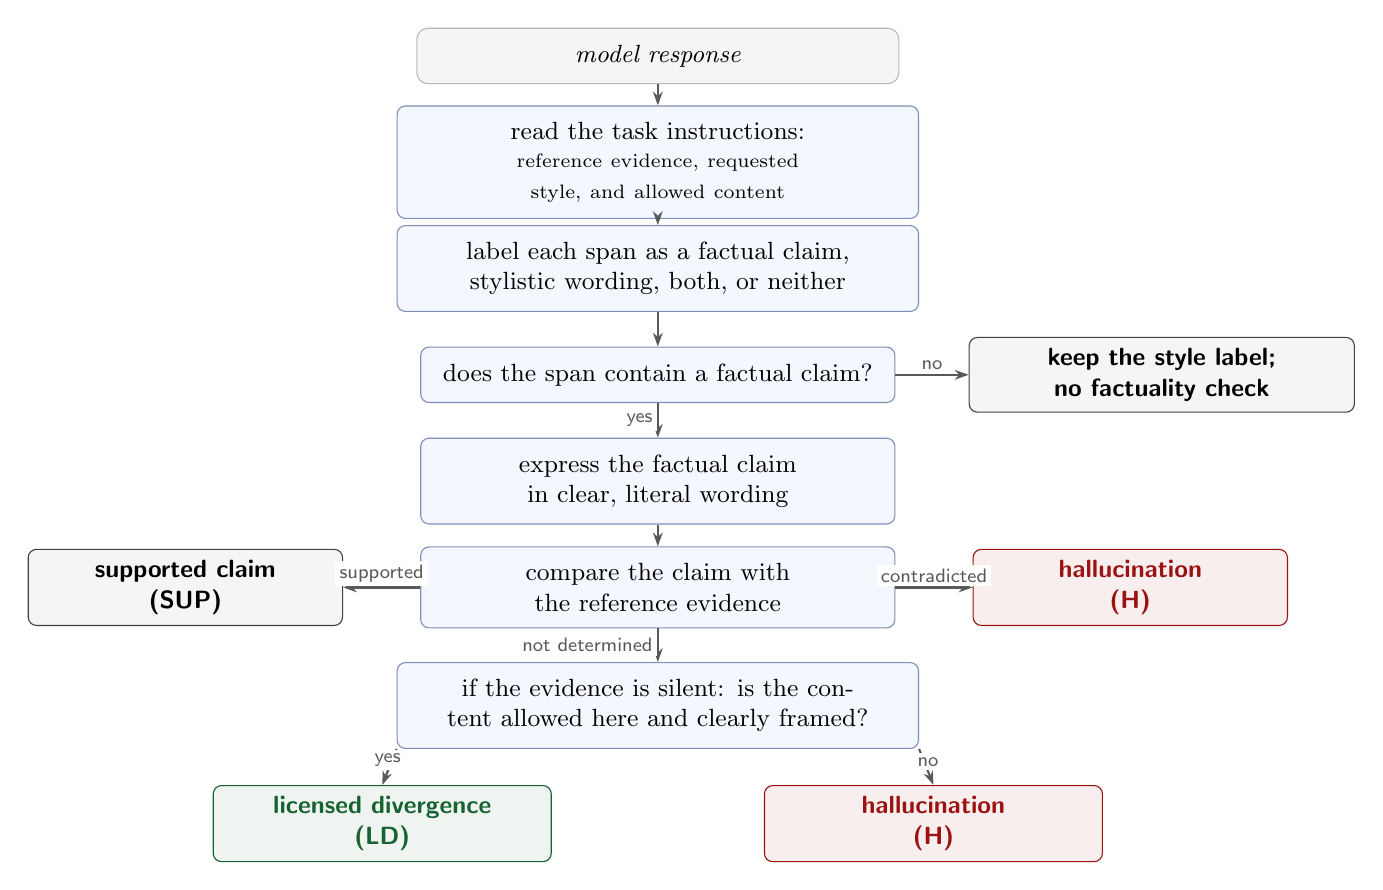
\begin{tikzpicture}[x=1cm,y=1cm]
  \node[input,text width=5.7cm] (response) at (0,0) {model response};
  \node[decision,text width=6.2cm] (contract) at (0,-1.35)
    {read the task instructions:\\[-1pt]{\scriptsize reference evidence, requested style, and allowed content}};
  \node[decision,text width=6.2cm] (label) at (0,-2.70)
    {label each span as a factual claim, stylistic wording, both, or neither};
  \node[decision,text width=5.6cm] (hasclaim) at (0,-4.05)
    {does the span contain a factual claim?};
  \node[verdict,text width=4.4cm,align=center] (styleonly) at (6.4,-4.05)
    {keep the style label;\\no factuality check};
  \node[decision,text width=5.6cm] (plainclaim) at (0,-5.40)
    {express the factual claim in clear, literal wording};
  \node[decision,text width=5.6cm] (evidence) at (0,-6.75)
    {compare the claim with the reference evidence};
  \node[verdict,text width=3.5cm,align=center] (sup) at (-6.0,-6.75)
    {supported claim\\(\SUP)};
  \node[verdictH,text width=3.5cm,align=center] (contradicted) at (6.0,-6.75)
    {hallucination\\(\Hall)};
  \node[decision,text width=6.2cm] (permission) at (0,-8.25)
    {if the evidence is silent: is the content allowed here and clearly framed?};
  \node[verdictLD,text width=3.8cm,align=center] (licensed) at (-3.5,-9.75)
    {licensed divergence\\(\LD)};
  \node[verdictH,text width=3.8cm,align=center] (unlicensed) at (3.5,-9.75)
    {hallucination\\(\Hall)};
  \draw[arrow] (response) -- (contract);
  \draw[arrow] (contract) -- (label);
  \draw[arrow] (label) -- (hasclaim);
  \draw[arrow] (hasclaim) -- node[edge,left]{yes} (plainclaim);
  \draw[arrow] (hasclaim.east) -- node[edge,above]{no} (styleonly.west);
  \draw[arrow] (plainclaim) -- (evidence);
  \draw[arrow] (evidence.west) -- node[edge,above]{supported} (sup.east);
  \draw[arrow] (evidence.east) -- node[edge,above]{contradicted} (contradicted.west);
  \draw[arrow] (evidence) -- node[edge,left]{not determined} (permission);
  \draw[arrow] (permission.south west) -- node[edge,above,pos=0.62]{yes} (licensed.north);
  \draw[arrow] (permission.south east) -- node[edge,above,pos=0.62]{no} (unlicensed.north);
\end{tikzpicture}}
\caption{\textbf{Plain-language span-to-claim evaluation procedure.}
The evaluator first reads the task instructions and labels the role of each span.
Stylistic wording without a factual claim is retained but not fact-checked.
Each factual claim is rewritten in a clear form and compared with the reference evidence.
When the evidence is silent, the claim is accepted as licensed divergence only if the task allows it in that context and the response presents it as required.}
\label{fig:decision}
\end{figure*}

\subsection{Representative contracts}

Table~\ref{tab:contracts} applies the rule to representative prompts.
Each row specifies one contract and evaluates the claims recovered from one output span.

\begin{table*}[t]
\centering
\small
\setlength{\tabcolsep}{5pt}
\renewcommand{\arraystretch}{1.15}
\caption{\textbf{Representative truth contracts and claim-level verdicts.}
$O$ is the reference evidence, $\sigma$ is the requested style level, $\kappa$ is the permission level, and $K$ is the full content-permission policy.
\SUP, \LD, and \Hall\ are claim-level verdicts; \SV\ is an auxiliary span flag.}
\label{tab:contracts}
\begin{tabularx}{\linewidth}{@{}P{0.18\linewidth}P{0.18\linewidth}YP{0.12\linewidth}P{0.17\linewidth}@{}}
\toprule
\textbf{Prompt} & \textbf{Contract} & \textbf{Output span} & \textbf{Label} & \textbf{Reason}\\
\midrule
Summarize this medical report & $O$: report; $\sigma=0$; $\kappa=0$ (factual only) & The patient has diabetes (absent from the report) & \Hall & Unknown and unlicensed\\
Explain photosynthesis like a poet, but keep the science accurate & $O$: scientific references; $\sigma=2$; $\kappa=0$ (factual only) & Chlorophyll catches sunlight, fueling the plant's sugar-making work & \SUP+\SV & Canonical claims supported; form marked\\
List possible causes and mark unestablished suggestions & $O$: clinical evidence; $\sigma=0$; $\kappa=1$ (limited divergence in diagnostic scope) & This could be early Lyme disease, but it requires testing & \LD & Unknown, in scope, and provisional\\
Write a story set in 1920s Paris & $O$: prompt constraints; $\sigma=1$; $\kappa=2$ (in-frame invention) & The fictional caf\'e Verdier opened at dawn & \LD & Invention inside the fictional frame\\
Write a story set in 1920s Paris & $O$: prompt and historical constraints; $\sigma=1$; $\kappa=2$ (in-frame invention) & A real named person made a fabricated statement, presented as biography & \Hall & Real-world claim outside scope\\
\bottomrule
\end{tabularx}
\end{table*}

\section{Purposive Mapping of a Diagnostic Gap}\label{sec:audit}

\subsection{Purposive mapping protocol}

We examined forty author-selected evaluation resources covering factual question answering, grounded generation, intent evaluation, creative writing, divergent thinking, and constrained problem solving.
The mapping is purposive rather than systematic.
It asks whether prominent examples from factuality and creativity research explicitly represent the variables in the proposed contract.

For each resource, we recorded five questions:
\begin{enumerate}
  \item Does the protocol specify a reference evidence source?
  \item Does it vary or score the requested style level while controlling claim content?
  \item Does it vary or score the permission to introduce unsupported content?
  \item Does it represent the scope of that permission?
  \item Does it score the required epistemic presentation?
\end{enumerate}
For the second question, we also recorded whether marked form is evaluated as a possible source of factuality-measurement error.

Appendix~\ref{app:mapping} expresses these observations in the framework's terms.
Each resource receives a coarse task-level code for its reference evidence $O$, its dominant requested style level $\sigma$, and its inferred permission level $\kappa$.
We use $\kappa=0$ for factual-only tasks, $\kappa=1$ for limited divergence constrained by explicit marking, feasibility, tests, or soundness, and $\kappa=2$ for invention inside a declared task frame.
An ``implicit'' code means that the level is inferred from the task design rather than represented as an independent evaluation variable.
The number estimates the breadth of permitted departure; it does not measure benchmark quality or replace the scope and presentation components of $K$.

The mapping was coded in a single pass by one author.
The inferred task profiles are interpretive annotations, not measurements reported by the original resources.
Our conclusions are therefore limited to this sample.
Independent recoding and a public codebook would be required before treating the mapping as a validated resource.
Appendix~\ref{app:mapping} lists the resources and their coarse inferred profiles.

\subsection{Observed pattern in the sample}

Table~\ref{tab:mapping-summary} summarizes the mapping at the level of resource groups.
The twenty-four strict factuality and faithfulness resources generally fix reference evidence, assume neutral wording ($\sigma=0$), and treat unsupported claims as errors under an inferred $\kappa=0$ policy.
The two closest intent or hallucination-taxonomy resources represent part of the problem but do not jointly score evidence, permission scope, and presentation.
Creative-writing resources more often request or reward marked language ($\sigma=1$ or $2$) and imply $\kappa=2$, but they generally do not encode $K$---including its scope and required epistemic presentation---as an independent variable.
Divergent-thinking resources also imply $\kappa=2$ but often do not control linguistic style; the five constrained creative-problem-solving resources instead combine mostly neutral form with a partial $\kappa=1$ policy based on feasibility or correctness.
These distributions are not paradoxical results about one capability: the resource groups evaluate different regions of the truth-contract space.
The main missing region is controlled evaluation that crosses $\sigma\in\{0,1,2\}$ with a fixed grounded-only policy, especially strongly marked but factually grounded language.
Within this author-coded sample, we did not identify a resource that jointly represents $O_p$, $\sigma_p$, and $K_p$ as independent evaluation variables.
We also did not identify a protocol that jointly evaluates $\sigma_p$-conditioned span typing, \SV\ placement, extracted claim sets, and downstream claim-level verdicts.

\begin{table*}[t]
\centering
\scriptsize
\renewcommand{\arraystretch}{1.12}
\caption{\textbf{Summary of the purposive mapping of forty resources.}
The counts describe the author-coded sample, not the full literature.
The columns summarize reference evidence, the inferred permission level $\kappa$, its scope and epistemic presentation, and control of the requested style level.
``Implicit'' means that the task design appears to assume a value without scoring it as an independent variable.}
\label{tab:mapping-summary}
\begin{tabularx}{\linewidth}{@{}YP{0.04\linewidth}P{0.14\linewidth}P{0.13\linewidth}P{0.09\linewidth}P{0.15\linewidth}P{0.14\linewidth}@{}}
\toprule
\textbf{Resource group} & \textbf{$n$} & \shortstack{\textbf{Reference}\\\textbf{evidence}} & \shortstack{\textbf{Inferred}\\\textbf{$\kappa$}} & \textbf{Scope} & \shortstack{\textbf{Epistemic}\\\textbf{presentation}} & \shortstack{\textbf{Inferred $\sigma$}\\\textbf{/ control}}\\
\midrule
Strict factuality / faithfulness & 24 & Usually fixed evidence & $0$; implicit & Not varied & Factual assertion expected & $0$; implicit\\
Intent / hallucination taxonomy & 2 & Partial or task-dependent & $0$--$2$; partial & Not jointly scored & Partly represented & $0$ dominant; not controlled\\
Creative generation / divergent thinking & 9 & Often rubric-based & $2$; implicit & Usually task-implied & Usually in-frame & Mixed: $1$--$2$ in writing; often uncontrolled in divergent thinking\\
Creative problem solving & 5 & Tests, environment, feasibility, or soundness & $1$; partial & Defined by task & Task-implied & $0$ dominant; implicit\\
\bottomrule
\end{tabularx}
\end{table*}

The sample also underrepresents strongly marked language under a strict factual contract.
Existing resources more often pair factual contracts with neutral language and creative contracts with marked language.
Examples include ``explain this scientific result like a poet, but keep every claim accurate.''
Such tasks can reveal whether a factuality verifier mistakes figurative wording for unsupported claim content.
Modern verification pipelines make this a plausible failure mode because claim decomposition, natural-language inference, and semantic similarity may all depend on the surface realization \citep{chen_menli_2023,aynetdinov_semscore_2024}.
This is a measurement hypothesis, not a prevalence result established by the present paper.

Figure~\ref{fig:profiles} organizes the target task profiles by requested style and breadth of permitted departure.

\begin{figure*}[t]
\centering
\resizebox{0.96\linewidth}{!}{%
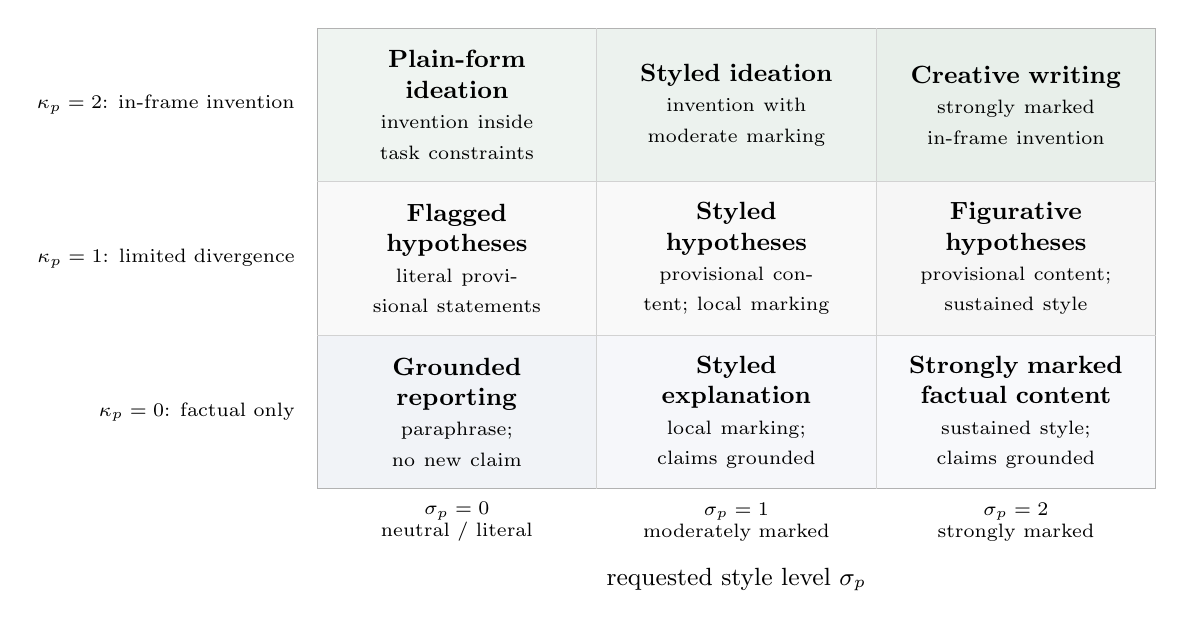
\begin{tikzpicture}[x=1cm,y=1cm,font=\small]
  \def\cw{3.55}
  \def\rh{1.95}
  \fill[clrB!6] (0,0) rectangle (\cw,\rh);
  \fill[clrB!4] (\cw,0) rectangle (2*\cw,\rh);
  \fill[clrB!3] (2*\cw,0) rectangle (3*\cw,\rh);
  \fill[gray!5] (0,\rh) rectangle (\cw,2*\rh);
  \fill[gray!5] (\cw,\rh) rectangle (2*\cw,2*\rh);
  \fill[gray!7] (2*\cw,\rh) rectangle (3*\cw,2*\rh);
  \fill[clrLD!7] (0,2*\rh) rectangle (\cw,3*\rh);
  \fill[clrLD!8] (\cw,2*\rh) rectangle (2*\cw,3*\rh);
  \fill[clrLD!10] (2*\cw,2*\rh) rectangle (3*\cw,3*\rh);
  \draw[gray!60] (0,0) rectangle (3*\cw,3*\rh);
  \draw[gray!35] (\cw,0)--(\cw,3*\rh);
  \draw[gray!35] (2*\cw,0)--(2*\cw,3*\rh);
  \draw[gray!35] (0,\rh)--(3*\cw,\rh);
  \draw[gray!35] (0,2*\rh)--(3*\cw,2*\rh);
  \node[align=center,text width=3.15cm] at (0.5*\cw,0.5*\rh)
    {\textbf{Grounded reporting}\\{\scriptsize paraphrase; no new claim}};
  \node[align=center,text width=3.15cm] at (1.5*\cw,0.5*\rh)
    {\textbf{Styled\\explanation}\\{\scriptsize local marking; claims grounded}};
  \node[align=center,text width=3.15cm] at (2.5*\cw,0.5*\rh)
    {\textbf{Strongly marked\\factual content}\\{\scriptsize sustained style; claims grounded}};
  \node[align=center,text width=3.15cm] at (0.5*\cw,1.5*\rh)
    {\textbf{Flagged\\hypotheses}\\{\scriptsize literal provisional statements}};
  \node[align=center,text width=3.15cm] at (1.5*\cw,1.5*\rh)
    {\textbf{Styled\\hypotheses}\\{\scriptsize provisional content; local marking}};
  \node[align=center,text width=3.15cm] at (2.5*\cw,1.5*\rh)
    {\textbf{Figurative hypotheses}\\{\scriptsize provisional content; sustained style}};
  \node[align=center,text width=3.15cm] at (0.5*\cw,2.5*\rh)
    {\textbf{Plain-form ideation}\\{\scriptsize invention inside task constraints}};
  \node[align=center,text width=3.15cm] at (1.5*\cw,2.5*\rh)
    {\textbf{Styled ideation}\\{\scriptsize invention with moderate marking}};
  \node[align=center,text width=3.15cm] at (2.5*\cw,2.5*\rh)
    {\textbf{Creative writing}\\{\scriptsize strongly marked in-frame invention}};
  \node[font=\scriptsize,align=center] at (0.5*\cw,-0.42){$\sigma_p=0$\\neutral / literal};
  \node[font=\scriptsize,align=center] at (1.5*\cw,-0.42){$\sigma_p=1$\\moderately marked};
  \node[font=\scriptsize,align=center] at (2.5*\cw,-0.42){$\sigma_p=2$\\strongly marked};
  \node[font=\small] at (1.5*\cw,-1.15){requested style level $\sigma_p$};
  \node[font=\scriptsize,anchor=east] at (-0.16,0.5*\rh){$\kappa_p=0$: factual only};
  \node[font=\scriptsize,anchor=east] at (-0.16,1.5*\rh){$\kappa_p=1$: limited divergence};
  \node[font=\scriptsize,anchor=east] at (-0.16,2.5*\rh){$\kappa_p=2$: in-frame invention};
\end{tikzpicture}}
\caption{\textbf{Conceptual task-design space.}
The grid crosses three content-permission levels with the three requested style levels, $\sigma_p\in\{0,1,2\}$.
Each cell is an illustrative task profile, not an empirical frequency or quality ranking.
A higher $\kappa_p$ broadens the type of departure that a task may permit, but scope and presentation constraints still apply.
A higher $\sigma_p$ changes the requested style level but does not license unsupported claims.}
\label{fig:profiles}
\end{figure*}

\subsection{Why unsupported generation is not the target}

Formal work suggests that some errors remain possible for sufficiently general models operating with incomplete evidence \citep{kalai_calibrated_2024,xu_hallucination_2024,banerjee_llms_2024}.
This does not imply a constant deployment error rate \citep{suzuki_negligible_2025}.
For our position, the main point is operational: suppressing every departure from observed evidence would also suppress hypotheses and in-frame invention.
Evaluation should instead reduce unlicensed departures (\Hall), preserve licensed ones (\LD), and retain supported content at the requested $\sigma_p$ level \citep{banerjee_does_2025,sun_hallucinating_2024,he_shakespearean_2025}.

\section{Worked Cases}\label{sec:cases}

The following cases illustrate how one or more contract components affect the analysis.
They are conceptual demonstrations rather than measurements.
Case A uses a documented summarization pattern; Cases B--E are constructed contrasts involving frame, permission, scope, presentation, and style-conditioned claim typing.

\paragraph{Case A: changing the reference evidence}
In XSum, an extrinsic but factual summary statement may be absent from the source document while being correct against external evidence \citep{maynez_faithfulness_2020}.
With $O=$ source document and grounded-only $K$, the statement is unsupported and receives \Hall.
With $O=$ an external evidence set that entails the same claim, it receives \SUP.
The surface text does not change; the reference evidence does.

\paragraph{Case B: changing the discourse frame}
The caf\'e sentence in Figure~\ref{fig:flip} is \Hall\ when interpreted as a real-world historical assertion under a grounded QA contract.
Under a declared fictional frame, the corresponding fictional-world claim is in scope and receives \LD.
The example holds the wording fixed while changing its contextualized claim and content-permission policy.

\paragraph{Case C: changing the epistemic presentation}
Suppose the available evidence cannot determine whether a tool supports several input formats.
Under a grounded contract, presenting support as an established fact receives \Hall.
Under a hypothesis-generation contract, a qualified statement such as ``the tool may support several formats, but this requires version-specific verification'' can receive \LD.
The canonical claim is preserved, but the content-permission policy and epistemic presentation differ.

\paragraph{Case D: testing a scope boundary}
A fictional frame does not license every false statement placed inside a story.
If a response attributes a fabricated biographical claim to a real named person and presents it as real history, the claim falls outside the fictional scope and remains \Hall.
Permission is limited by $\Gamma_p$.

\paragraph{Case E: changing claim type under requested style level}
Under $\sigma_p=0$, ``chlorophyll absorbs sunlight that powers sugar production'' has $\widehat\sigma=0$ and is analyzed as claim-only: its supported claims receive \SUP\ and $z_{\sigma_p}=0$.
Under $\sigma_p=2$, ``chlorophyll catches sunlight, fueling the plant's sugar-making work'' has $\widehat\sigma=2$ and is analyzed as mixed: the same canonical claims remain supported, while the marked realization receives $z_{\sigma_p}=1$ and is reported as \SUP+\SV.
If an evaluator extracts a literal pseudo-claim from the figurative wording, a subsequent \Hall\ label reflects an extraction error, not a factual defect in the intended claim.

\begin{table}[t]
\centering
\small
\setlength{\tabcolsep}{4pt}
\renewcommand{\arraystretch}{1.13}
\caption{\textbf{Worked cases illustrating contract-dependent verdicts.}
Each contrast may change one or more components.
\SUP, \LD, and \Hall\ are claim-level verdicts; \SV\ is an auxiliary span flag.}
\label{tab:cases}
\begin{tabular}{@{}cP{0.26\columnwidth}P{0.29\columnwidth}P{0.29\columnwidth}@{}}
\toprule
\textbf{Case} & \textbf{Main contrast} & \textbf{First condition} & \textbf{Second condition}\\
\midrule
A & Evidence $O$ & Source-only: \Hall & External evidence entails claim: \SUP\\
B & Frame and $K$ & Historical QA: \Hall & Fictional frame: \LD\\
C & Mode and presentation & Asserted as verified: \Hall & Licensed and flagged: \LD\\
D & Scope $\Gamma$ & In-frame invention: \LD & Real-world claim outside scope: \Hall\\
E & Requested and observed style levels & $\sigma=\widehat\sigma=0$: claim-only, \SUP & $\sigma=\widehat\sigma=2$: mixed, \SUP+\SV\\
\bottomrule
\end{tabular}
\end{table}

\section{Research Agenda}\label{sec:agenda}

The framework motivates three empirical priorities.

\textbf{1. Contract annotation and reliability.}
Benchmarks should annotate the reference evidence $O_p$, the three-level requested style level $\sigma_p$, the observed style level $\widehat\sigma$, permission level $\kappa_p$, scope, and epistemic presentation separately.
A public codebook should define contextualized claims, claim-preserving style variation, and evidence states.
Reliability should be reported for each layer, and annotator disagreement should be preserved when prompts are ambiguous.
Contract inference must also resolve conflicts among user prompts, system instructions, domain rules, and safety policies.

\textbf{2. Controlled benchmark design.}
A diagnostic benchmark should cross $\kappa_p\in\{0,1,2\}$ with $\sigma_p\in\{0,1,2\}$ while holding canonical claims as stable as possible.
Expert-adjudicated triplets should express the same claim in neutral, moderately marked, and strongly marked forms.
Evaluation should report span type, observed-style accuracy, \SV\ placement, claim-set equivalence, evidence state, and final verdict.
A successful evaluator need not produce identical raw extractions across styles; it should recover equivalent canonical claims and stable verdicts after matching.
The mapping in Appendix~\ref{app:mapping} provides possible comparators, not a validated benchmark.

\textbf{3. Mitigation that preserves licensed divergence and factual style.}
Retrieval, verification, abstention, and constrained decoding should be assessed on three outcomes: reducing \Hall\ under grounded contracts, preserving useful \LD\ under permissive contracts, and preserving supported content at $\sigma_p=1$ or $2$.
Usefulness should remain a separate score with its own uncertainty \citep{acar_creativity_2019,marco_reader_2025}.
One aggregate hallucination rate cannot represent these objectives.

\section{Discussion}\label{sec:discussion}

\subsection{Evaluation implications}

Contract-aware evaluation separates claim-level verdicts from output-level objectives.
At claim level, a departure is supported, hallucinated, or licensed.
At span level, \SV\ is an orthogonal flag: it may occur alone or accompany any claim-level verdict when stylistic material and claim content coexist.
At output level, a response may still be too conservative for a creative task even when it contains no \Hall.
Likewise, a response may remain supported but reduce a requested $\sigma_p=2$ style to neutral prose.
These are output-level task-compliance failures, not new claim labels.
Conversely, satisfying $\sigma_p=2$ does not excuse a fabricated claim under a grounded-only $K_p$.
Reporting claim-level verdicts and style compliance separately makes ``creative and factual when required'' an evaluable target.

The framework also separates verdict from severity.
A false drug dose and a wrong trivia date can both receive \Hall, but their costs differ.
Severity should weight the penalty after the contractual verdict rather than determine whether a violation occurred.

\subsection{Limitations}

The framework's limitations fall into three groups.
First, contract specification is partly normative: evaluators may disagree about the evidence source, permission boundary, or authority of user, system, safety, legal, and domain instructions.
The present framework is also prompt-centered and does not model how a contract changes across dialogue turns.

Second, claim extraction remains difficult under metaphor, irony, hypothesis, and fiction.
The three-level $\sigma_p$ scheme is a provisional discretization, and neither its thresholds nor the distinction between requested and observed style levels has been validated with human annotation.
The $\kappa_p$ scale is likewise provisional: it orders breadth of permission, but cannot replace task-specific scope and presentation rules.
The \LD\ rule and usefulness score also require reliability studies.

Third, the literature mapping is purposive and author-coded.
It identifies a pattern in the selected sample but cannot support prevalence claims about the full literature.
These limits restrict the present framework and motivate the empirical program above.

\section{Conclusion}\label{sec:conclusion}

Hallucination is not a context-free property of a sentence.
It is a claim-level verdict relative to a task's reference evidence, requested style level, and content-permission policy.
The truth contract $\TC(p)=(O_p,\sigma_p,K_p)$ separates these components.
An unknown claim is \LD\ only when it falls within the permitted scope and uses the required epistemic presentation; otherwise it is \Hall.
Usefulness, severity, and style compliance remain separate.

The purposive mapping suggests that these variables are rarely represented together in the resources we examined.
The worked cases show why each variable matters.
The next step is to validate contract-guided span typing, measure verdict stability after claim matching, and test whether mitigation can reduce \Hall\ while preserving \LD\ and factually grounded style.

\appendix

\appendixsection{Formal Decision Rule}\label{app:formal}

For a surface span $s$ produced under prompt $p$, let $\TC(p)=(O_p,\sigma_p,K_p)$ and define the contract-guided analysis
\[
\mathcal X_{\sigma_p}(s,p)
=
\bigl(\mathcal C_{\sigma_p}(s,p),\widehat\sigma(s,p),z_{\sigma_p}(s,p)\bigr),
\]
where $\mathcal C_{\sigma_p}(s,p)$ is a possibly empty set of contextualized claims, $\widehat\sigma(s,p)$ is the observed style level, and $z_{\sigma_p}(s,p)$ is the \SV\ flag.
If $\mathcal C_{\sigma_p}=\varnothing$, the span exits factual verification; it is SV-only when $z_{\sigma_p}=1$ and other when $z_{\sigma_p}=0$.
If $\mathcal C_{\sigma_p}\neq\varnothing$, each $c\in\mathcal C_{\sigma_p}$ is verified; when $z_{\sigma_p}=1$, \SV\ is retained as an auxiliary annotation beside the claim-level verdict.

For every extracted claim, define
\[
E(c,O_p)\in\{\textsc{entailed},\textsc{contradicted},\textsc{unknown}\},
\]
let $r(c,s)$ denote the realization of claim $c$ in span $s$, and let
\begin{align*}
L(c,K_p)&=\mathbf{1}[\kappa_p\text{ permits }c\text{ within }\Gamma_p],\\
M(c,s,K_p)&=\mathbf{1}[r(c,s)\text{ satisfies the epistemic presentation }\rho_p].
\end{align*}
The verdict is
\[
V(c\mid p)=
\begin{cases}
\SUP & E(c,O_p)=\textsc{entailed},\\
\LD & E(c,O_p)=\textsc{unknown},\ L(c,K_p)=1,\ M(c,s,K_p)=1,\\
\Hall & \text{otherwise.}
\end{cases}
\]
Usefulness is a separate, task-dependent score $U(c,p)$ defined by the evaluation protocol.

An automatic evaluator should report three diagnostics separately.
\emph{Type error} measures incorrect assignment of other, SV-only, claim-only, or mixed.
\emph{Claim error} measures dropped or spurious canonical claims.
\emph{Verdict instability} measures whether claim-matched variants receive different verdicts when $O$ and $K$ are fixed.
These diagnostics require a benchmark distribution and expert-adjudicated matches before they can be estimated as error rates.

The central claim can be stated for one canonical claim and one reference evidence source:
\[
\begin{gathered}
\exists c,p_1,p_2:\quad O_{p_1}=O_{p_2}=O,\\
E(c,O)=\textsc{unknown},\\
V(c\mid p_1)=\Hall\ \land\ V(c\mid p_2)=\LD.
\end{gathered}
\]
The canonical claim and evidence state are fixed; the content-permission policy and epistemic presentation differ.
This is a claim about contract-dependent verdicts, not relative truth.

\appendixsection{Resource Mapping}\label{app:mapping}

Tables~\ref{tab:full-mapping-factual-a}--\ref{tab:full-mapping-creative} list the forty resources used in the purposive mapping.
Each row encodes the reference evidence $O$, the dominant requested style level $\sigma$, and the inferred permission level $\kappa$.
The $\sigma$ column uses the paper's three levels; ``not controlled'' means that style is neither fixed nor scored as a distinct variable.
The $\kappa$ column uses $0$ for factual only, $1$ for limited divergence, and $2$ for in-frame invention.
``Implicit'' means that the level is inferred from the task design, while ``partial'' means that the resource encodes a constraint such as correctness or feasibility without representing the full policy $(\kappa,\Gamma,\rho)$.
Thus, an implicit $\kappa=2$ code does not mean that a benchmark explicitly annotates the content-permission policy; it means that invention is needed or accepted by the task although its permission boundary is not independently evaluated.
The task profiles are coarse author annotations inferred from the original protocols, not labels reported by those resources.
They require a public codebook and independent recoding before release as a validated dataset.

\begin{table*}[t]
\centering
\scriptsize
\setlength{\tabcolsep}{4pt}
\renewcommand{\arraystretch}{0.98}
\caption{\textbf{Factuality and faithfulness resources in the purposive mapping (part I).}
The recurring profile is fixed reference evidence, implicit $\sigma=0$, and inferred factual-only permission ($\kappa=0$).
No listed resource crosses a grounded-only policy with controlled $\sigma=1$ or $2$.
These are author-coded profiles, not labels reported by the original resources.}
\label{tab:full-mapping-factual-a}
\begin{tabularx}{0.98\linewidth}{@{}P{0.23\textwidth}P{0.18\textwidth}P{0.20\textwidth}P{0.11\textwidth}Y@{}}
\toprule
\textbf{Resource} & \textbf{Task} & \textbf{$O$: reference evidence or rubric} & \textbf{Inferred $\sigma$} & \textbf{Inferred $\kappa$ / status}\\
\midrule
\multicolumn{5}{l}{\textbf{Strict factuality and faithfulness}}\\
FEVER \citep{thorne_fever_2018} & Fact checking & Wikipedia evidence & $0$ (implicit) & $0$ (implicit)\\
TruthfulQA \citep{lin_truthfulqa_2022} & Factual QA & External factual reference & $0$ (implicit) & $0$ (implicit)\\
PopQA \citep{mallen_when_2023} & Long-tail QA & Wikidata & $0$ (implicit) & $0$ (implicit)\\
SimpleQA \citep{wei_measuring_2024} & Factual QA & External factual reference & $0$ (implicit) & $0$ (implicit)\\
TriviaQA \citep{joshi_triviaqa_2017} & Reading QA & Evidence documents & $0$ (implicit) & $0$ (implicit)\\
DefAn \citep{rahman_defan_2024} & Factual QA & External factual reference & $0$ (implicit) & $0$ (implicit)\\
HaluEval \citep{li_halueval_2023} & QA and summarization & World/reference context & $0$ (implicit) & $0$ (implicit)\\
FactBench \citep{bayat_factbench_2024} & Factual QA & Retrieved evidence & $0$ (implicit) & $0$ (implicit; undecidable retained)\\
HalluLens \citep{bang_hallulens_2025} & Factual QA & Task-specific evidence & $0$ (implicit) & $0$ (implicit)\\
FRANK \citep{pagnoni_understanding_2021} & Summarization & Source documents & $0$ (implicit) & $0$ (implicit)\\
QAGS \citep{wang_asking_2020} & Summarization & Source documents & $0$ (implicit) & $0$ (implicit)\\
SummEval \citep{fabbri_summeval_2021} & Summarization & Source documents & $0$ (implicit) & $0$ (implicit)\\
XSum \citep{narayan_xsum_2018} & Summarization & BBC source & $0$ (implicit) & $0$ (implicit)\\
\bottomrule
\end{tabularx}
\end{table*}

\begin{table*}[t]
\centering
\scriptsize
\setlength{\tabcolsep}{4pt}
\renewcommand{\arraystretch}{0.98}
\caption{\textbf{Factuality, faithfulness, and adjacent resources in the purposive mapping (part II).}
The coding follows Table~\ref{tab:full-mapping-factual-a}: $\kappa=0$ denotes factual only, and ``partial'' denotes incomplete representation of the content-permission policy.
These are author-coded profiles, not labels reported by the original resources.}
\label{tab:full-mapping-factual-b}
\begin{tabularx}{0.98\linewidth}{@{}P{0.23\textwidth}P{0.18\textwidth}P{0.20\textwidth}P{0.11\textwidth}Y@{}}
\toprule
\textbf{Resource} & \textbf{Task} & \textbf{$O$: reference evidence or rubric} & \textbf{Inferred $\sigma$} & \textbf{Inferred $\kappa$ / status}\\
\midrule
\multicolumn{5}{l}{\textbf{Strict factuality and faithfulness (continued)}}\\
CNN/DailyMail \citep{hermann_teaching_2015} & Summarization & News source & $0$ (implicit) & $0$ (implicit)\\
DelusionQA \citep{sadat_delucionqa_2023} & Domain QA & Manuals & $0$ (implicit) & $0$ (implicit)\\
HaluQA \citep{cheng_evaluating_2023} & Long-form QA & External factual reference & $0$ (implicit) & $0$ (implicit)\\
BIG-Bench \citep{srivastava_beyond_2023} & Multi-task reasoning & Task gold & $0$ (implicit) & $0$ (implicit)\\
BIG-Bench Hard \citep{suzgun_challenging_2023} & Reasoning & Task gold & $0$ (implicit) & $0$ (implicit)\\
CR-LLM \citep{li_cr-llm_2024} & Concept reasoning & Gold concepts/context & $0$ (implicit) & $0$ (implicit)\\
HotpotQA \citep{yang_hotpotqa_2018} & Multi-hop QA & Wikipedia & $0$ (implicit) & $0$ (implicit)\\
HypoTermQA \citep{uluoglakci_hypotermqa_2024} & Hypothetical QA & Task/world reference & $0$ (implicit) & $0$ (implicit)\\
HalluRAG \citep{ridder_hallurag_2025} & RAG QA & Retrieved Wikipedia & $0$ (implicit) & $0$ (implicit)\\
ToolQA \citep{zhuang_toolqa_2023} & Tool-use QA & Tools and APIs & $0$ (implicit) & $0$ (implicit)\\
RealTimeQA \citep{kasai_realtime_2024} & Real-time QA & Current evidence & $0$ (implicit) & $0$ (implicit)\\
\midrule
\multicolumn{5}{l}{\textbf{Closest intent and hallucination taxonomies}}\\
FaithQA \citep{hao_faithqa_2025} & Intent verification & Query constraints & $0$ dominant; not controlled & $0$--$1$ (partial: intent constraints)\\
HIC-Bench \citep{yang_hicbench_2025} & Hallucination typing & Task-dependent & $0$ dominant; not controlled & $0$--$2$ (partial: hallucination types)\\
\bottomrule
\end{tabularx}
\end{table*}

\begin{table*}[t]
\centering
\scriptsize
\setlength{\tabcolsep}{4pt}
\renewcommand{\arraystretch}{0.98}
\caption{\textbf{Creativity and constrained problem-solving resources in the purposive mapping.}
Creative-writing resources tend toward $\sigma=1$--$2$ with task-implied $\kappa=2$, whereas divergent-thinking tasks often leave style uncontrolled.
Constrained problem-solving resources mostly use neutral form and partial $\kappa=1$ constraints.
The profiles are author annotations inferred from task design, not variables reported by the original resources.}
\label{tab:full-mapping-creative}
\begin{tabularx}{0.98\linewidth}{@{}P{0.23\textwidth}P{0.18\textwidth}P{0.20\textwidth}P{0.11\textwidth}Y@{}}
\toprule
\textbf{Resource} & \textbf{Task} & \textbf{$O$: reference evidence or rubric} & \textbf{Inferred $\sigma$} & \textbf{Inferred $\kappa$ / status}\\
\midrule
\multicolumn{5}{l}{\textbf{Creative generation and divergent thinking}}\\
CreativityPrism \citep{hou_creativityprism_2025} & Multi-task creativity & Task-specific rubrics & Mixed; not isolated & $2$ (implicit)\\
LitBench \citep{fein_litbench_2025} & Story evaluation & Human preferences & $1$--$2$ (implicit) & $2$ (implicit)\\
Short Story \citep{ismayilzada_evaluating_2025} & Story generation & Semantic/human criteria & $1$--$2$ (implicit) & $2$ (implicit)\\
WritingBench \citep{wu_writingbench_2025} & Creative writing & Rubric/human criteria & $1$--$2$ (style scored) & $2$ (implicit)\\
Art-or-Artifice / TTCW \citep{chakrabarty_art_2024} & Creative writing & Expert rubric & $1$--$2$ (implicit) & $2$ (implicit)\\
Automated DT scoring \citep{organisciak_beyond_2023} & Divergent thinking & Automated rubric & Not controlled & $2$ (implicit)\\
Verbal Creativity \citep{dinu_testing_2025} & Divergent thinking & TTCT & Not controlled & $2$ (implicit)\\
Automated Creativity \citep{li_automated_2025} & Creative writing & Reference texts & $1$--$2$ (implicit) & $2$ (implicit)\\
Hallucinating Narratives \citep{sun_hallucinating_2024} & Controlled story/reasoning & Mixed evidence/rubric & $1$--$2$ (implicit) & $2$ (partial; mixed support)\\
\midrule
\multicolumn{5}{l}{\textbf{Constrained creative problem solving}}\\
MacGyver \citep{tian_macgyver_2025} & Problem solving & Human feasibility & $0$ (implicit) & $1$ (partial: feasibility)\\
EscapeBench \citep{qian_escapebench_2025} & Agent puzzles & Environment state & $0$ (implicit) & $1$ (partial: correctness)\\
CreativEval \citep{delorenzo_creativeval_2024} & Code generation & Specification/tests & $0$ (implicit) & $1$ (partial: correctness)\\
NeoCoder \citep{lu_benchmarking_2025} & Code generation & Unit tests & $0$ (implicit) & $1$ (partial: correctness)\\
Math Creativity \citep{ye_assessing_2024} & Math problem solving & Human soundness & $0$ (implicit) & $1$ (partial: soundness)\\
\bottomrule
\end{tabularx}
\end{table*}

\bibliography{references}

\end{document}
